% Chapter Template

%\section{Mechanism and Design} % Main chapter title

%\label{Chapter8} % Change X to a consecutive number; for referencing this chapter elsewhere, use \ref{ChapterX}\ref{ChapterX}\ref{ChapterX}\ref{ChapterX}

%----------------------------------------------------------------------------------------
%	SECTION 1
%----------------------------------------------------------------------------------------

\section{Mechanism and Design}
\subsection{Output Motors}
A paramount challenge in the design of handheld cable-driven devices lies in the selection of the actuation unit. The motor must satisfy two critical, and often conflicting, requirements: it must be extremely lightweight to maintain a low overall device mass and ensure ergonomic usability, while simultaneously being capable of delivering sufficient torque to reliably tension the driving cables for both grasping and manipulation tasks. High torque output is essential to overcome friction in the cable pathways, generate the necessary gripping force, and provide adequate acceleration for precise movements.

After a comprehensive evaluation of available options,  Feetech STS3032, a smart servo was selected for this application. This choice was driven by its exceptional  ratio over performance-to-weight and integrated control architecture. Key factors influencing this decision include:
The STS3032 servo weighs a mere 9 grams, yet it delivers a substantial stall torque of 4.5 kg·cm. This high torque output ensures that the servo can generate significant tensile force in the cables, even when operating through small-diameter pulleys or under load, making it ideally suited for the demands of a surgical gripper.Unlike traditional pulse-width modulation (PWM) servos that require a dedicated control wire for each unit, the STS3032 utilizes a serial bus communication protocol. This architecture allows multiple servos to be daisy-chained and controlled via a single data line, drastically reducing the number of wires running through the device's handle. This reduction in cabling is a significant advantage for miniaturization, improving flexibility, simplifying assembly, and enhancing overall system reliability.

Another advantage of the this motor is that, as a smart servo, the STS3032 provides built-in feedback on parameters such as position, speed, and load. This enables closed-loop control strategies, which are critical for achieving the high positional accuracy and force sensitivity required for precise manipulation. The ability to read the motor's load provides valuable data for implementing basic force sensing, which can be used to prevent overloading and enable interactive control.

\subsection{Input Motors and Sensors}

The control philosophy for this cable-driven handheld device is based on replicating the user's hand movements with high fidelity and translating them into precise motions of the distal end-effector. This requires a sophisticated input system that can accurately capture the intent of the user's fingers while providing sufficient force feedback and stability.
\begin{figure}[htbp]
    \centering
    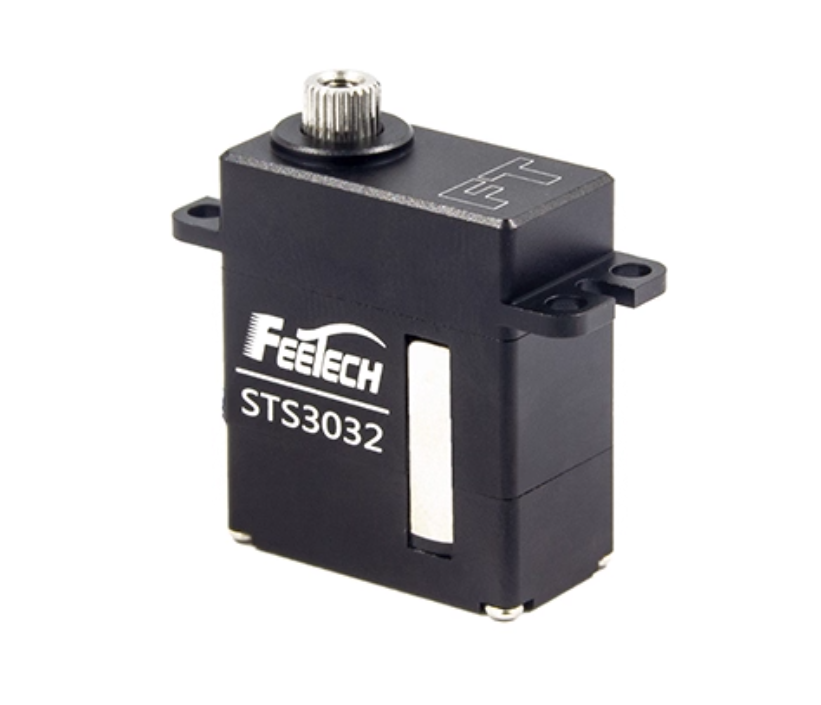
\includegraphics[width=0.7 \linewidth]{Figures/STS3032.png} 
    \caption{Feetech 3032 for output}
    \label{fig:81}
\end{figure}
For the input actuation, shown in Fig.\ref{fig:81}, the Feetech STS3009 servo was selected based on a different set of requirements. Weighing 40 grams and providing a stall torque of 0.3 Nm, this more powerful motor serves two essential functions in the input stage: it maintains mechanical equilibrium by resisting forces from the output tendons, thus offering a stable and responsive feel to the operator, and it helps filter out high-frequency physiological tremors or unintended jerks, ensuring that only deliberate commands are transmitted to the end-effector.
\begin{figure}[htbp]
    \centering
    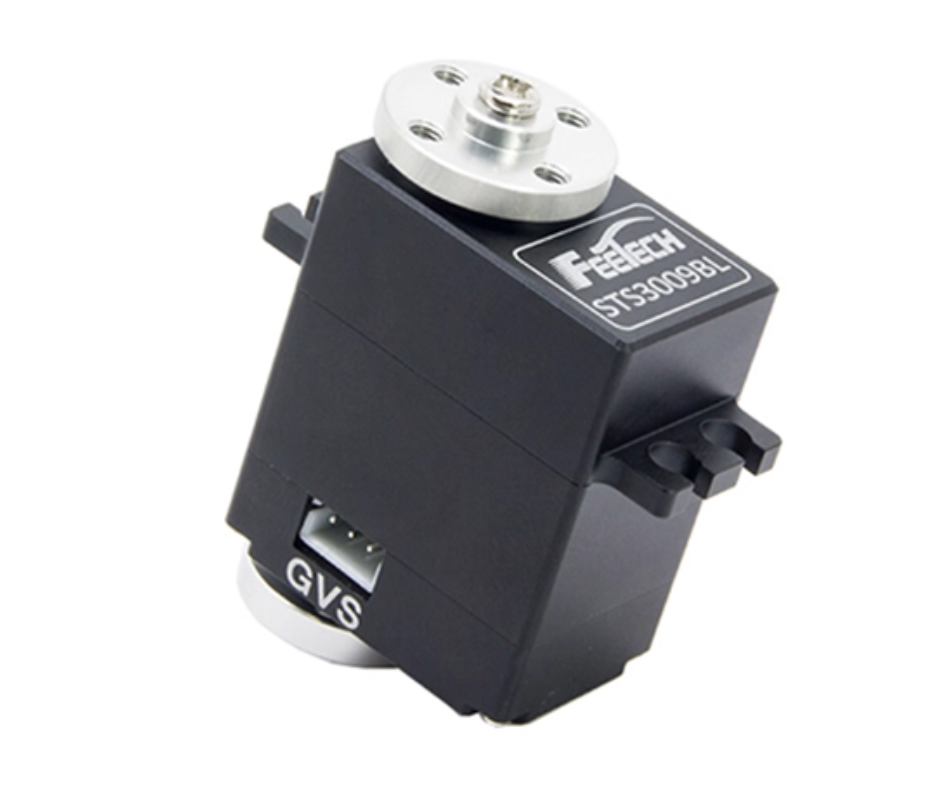
\includegraphics[width=0.7 \linewidth]{Figures/STS3009.png} 
    \caption{Feetech 3009 for wrist inputs}
    \label{fig:82}
\end{figure}


However, since the two input motors alone cannot fully capture all nuanced finger movements, a hybrid sensing strategy was implemented. Two AMS AS5600 magnetic rotary encoders were integrated into the input mechanism to directly and accurately detect the user’s intent. These sensors provide ultra-high 12-bit resolution and contactless sensing, enabling precise recognition of two distinct actions: the pinching gesture of the index finger and thumb, which controls grasping, and the rotational movement of the fingers, which is translated into in-plane rotation of the end-effector. This combination of robust actuation and high-resolution sensing creates an intuitive and stable human-machine interface suitable for delicate manipulation tasks.

\section{Cable Routing and Guidance System}
\subsection{Tip Design}
\begin{figure}[htbp]
    \centering
    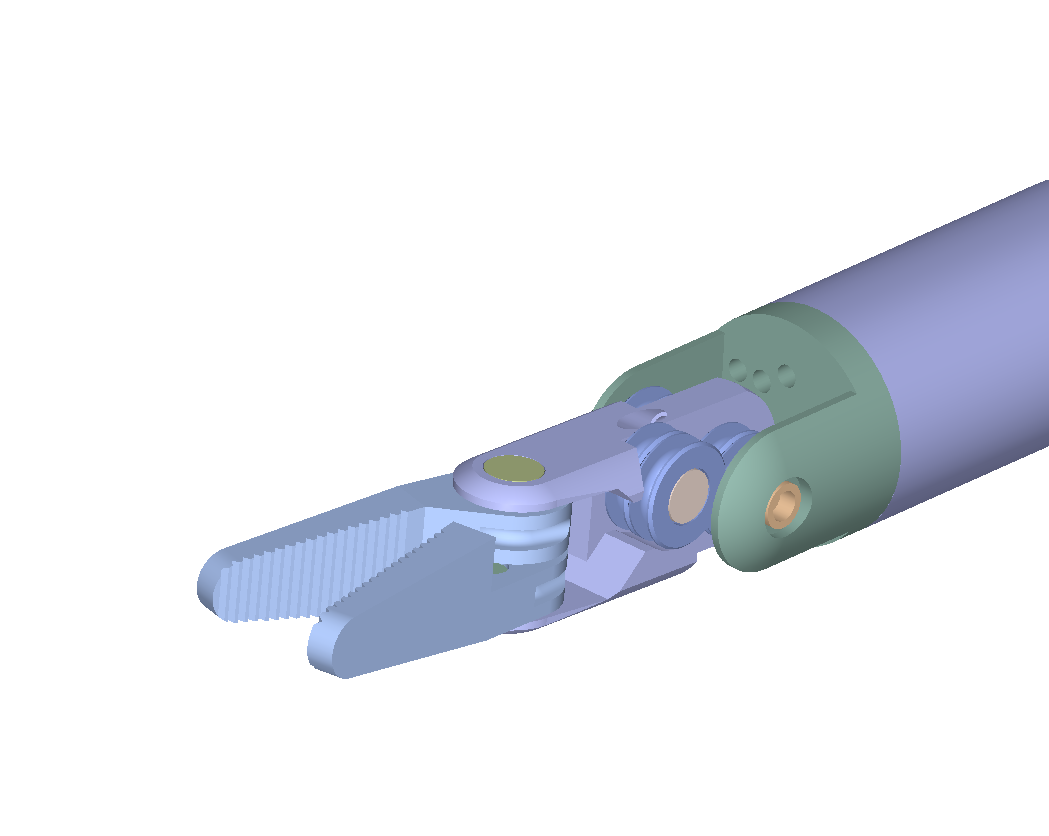
\includegraphics[width=0.7 \linewidth]{Figures/tip2.png} 
    \caption{Tip Design for Cable Guidance}
    \label{fig:83}
\end{figure}
In addition to motor performance, the accuracy and repeatability of the end-effector’s motion are highly dependent on precise cable guidance and sustained tension control. To ensure consistent behavior during operation, each cable must be constrained to move freely yet securely within a meticulously designed path, minimizing unwanted friction and slack.

A specialized tip assembly has been developed to fulfill these requirements. As shown in Fig.\ref{fig:83}, the four cables—grouped into two pairs, each controlling one jaw of the plier—are routed through custom-machined channels. These channels ensure that the cables remain aligned throughout the entire range of motion, avoiding cross-interference and reducing wear.

The two jaw components (fabricated in light pink) are mounted onto a central middle base (green). To further enhance cable stability and minimize friction, donut-shaped guides machined via CNC (purple) are integrated into the middle base. These spheres act as low-friction directional pulleys, maintaining cable position with high precision and reducing bending stress, thereby extending cable service life.

The main base housing (pink) is designed with precision-aligned holes that direct the cables perpendicularly toward the motors. This alignment is critical for maximizing force transmission efficiency and eliminating off-axis loading, which can introduce positioning errors and reduce system responsiveness.

Through this integrated approach—combining dedicated guiding channels, spherical contact points, and perpendicular alignment—the system achieves high repeatability, minimal hysteresis, and smooth force feedback, making it suitable for delicate manipulation tasks requiring fine motor control.

\subsection{Reel}

A fundamental challenge in cable-driven mechanisms lies in maintaining adequate tension during both winding and unwinding phases. In a conventional single-motor-single-cable configuration, unidirectional actuation presents a significant limitation: while rotation in one direction (e.g., clockwise) effectively pulls and tensions the cable, reverse rotation (counterclockwise) does not positively push the cable but often results in slack accumulation along the path. This leads to unpredictable response, reduced positional accuracy, and potential entanglements.

To address this issue, a paired-cable design has been implemented. The two cables corresponding to a single degree of freedom are affixed to the same axial shaft driven by one motor. This configuration effectively reforms the two independent cables into a continuous loop—functioning conceptually as a flexible drive belt. As a result, when the motor rotates in one direction, one cable is pulled while the other is simultaneously recovered, enabling bidirectional force transmission without slack accumulation.

\begin{figure}[htbp]
    \centering
    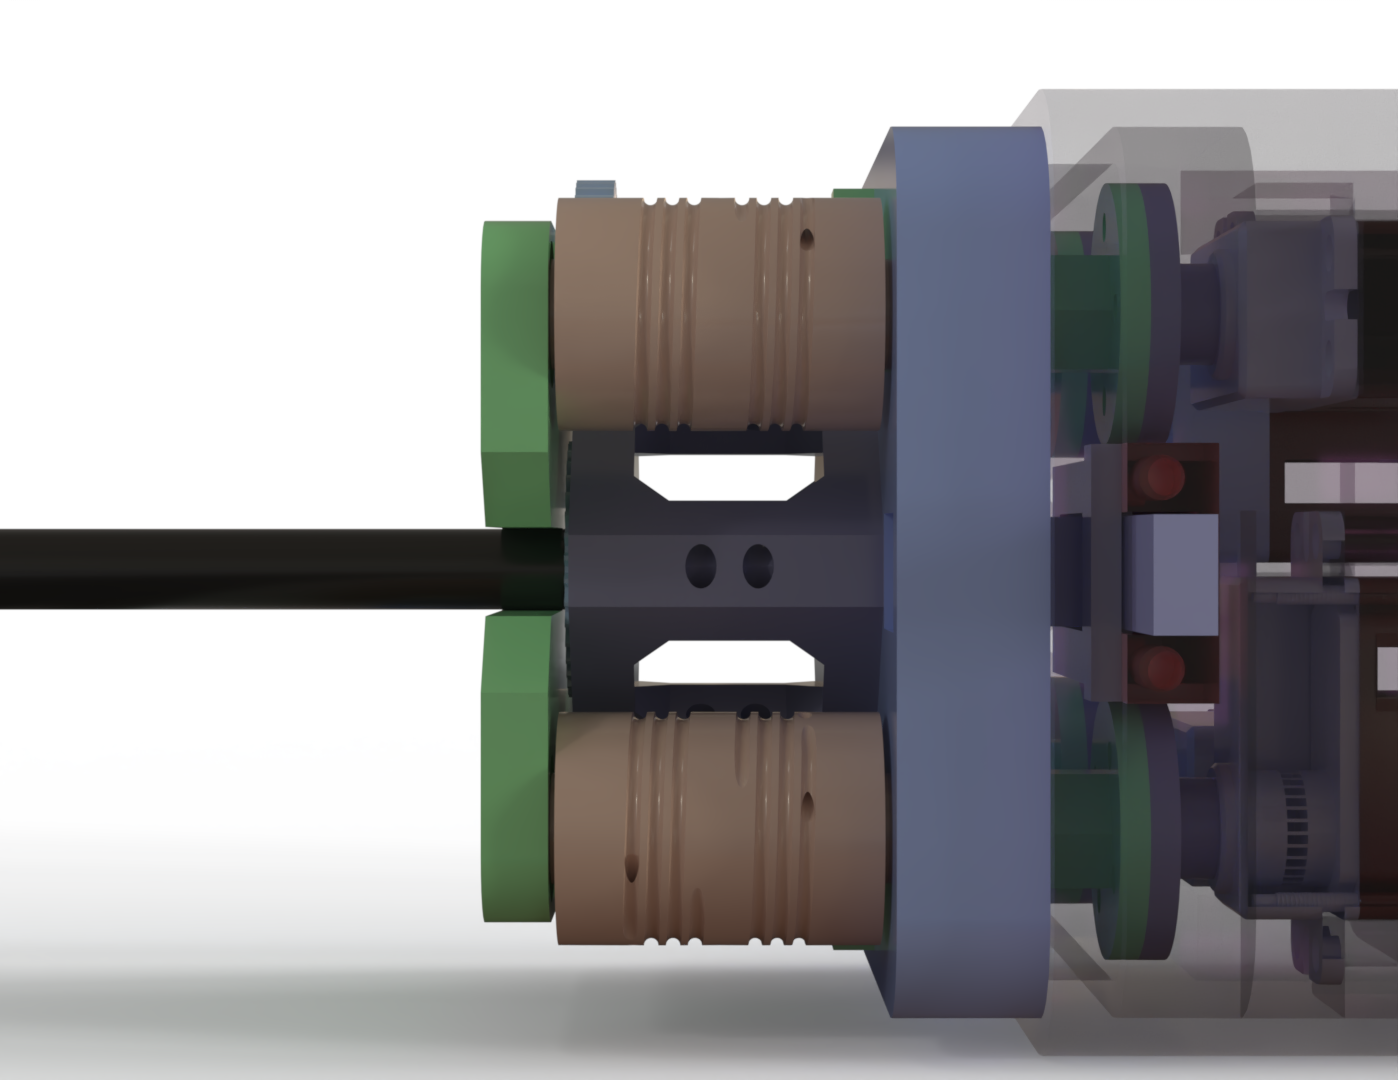
\includegraphics[width=0.7 \linewidth]{Figures/reel.png} 
    \caption{Reel Design and Winding Mechanism}
    \label{fig:84}
\end{figure}

The key to ensuring effective operation of this belt-like linkage is sustained cable tension. To achieve this, the reel assembly is split into two distinct components, each dedicated to one cable. These two reel pieces are mounted on the same shaft and are designed to rotate in opposite directions relative to each other. This counter-rotation ensures that one cable is wound while the other is unwound during actuation, maintaining constant tension across the system.

To prevent slippage and undesired loosening of the cables during operation, one-way bearings are incorporated into the reel mechanism. As the name implies, these bearings permit free rotation in one direction while locking in the opposite direction. This feature is critical for preserving tension integrity, especially during transitions in motor direction or under varying load conditions. The use of one-way bearings enhances system reliability, improves motion accuracy, and minimizes the need for manual tension adjustments.

\subsection{Motor Arrangement and Quick-Swap Mechanism}

As previously discussed, the STS3032 servos are employed as the driving motors for the cable reels. In practical surgical scenarios, various end-effector tips are often required throughout a single procedure. To accommodate this need, a quick-swap system has been integrated into the design, allowing for rapid and secure tip replacement without compromising system integrity.

To achieve a compact form factor suitable for handheld operation, the four motors are arranged in a rotational symmetry pattern within the main housing. This layout optimizes spatial efficiency while maintaining sufficient clearance for motor power and communication cables, thereby preventing interference and ensuring reliable connectivity.
\begin{figure}[htbp]
    \centering
    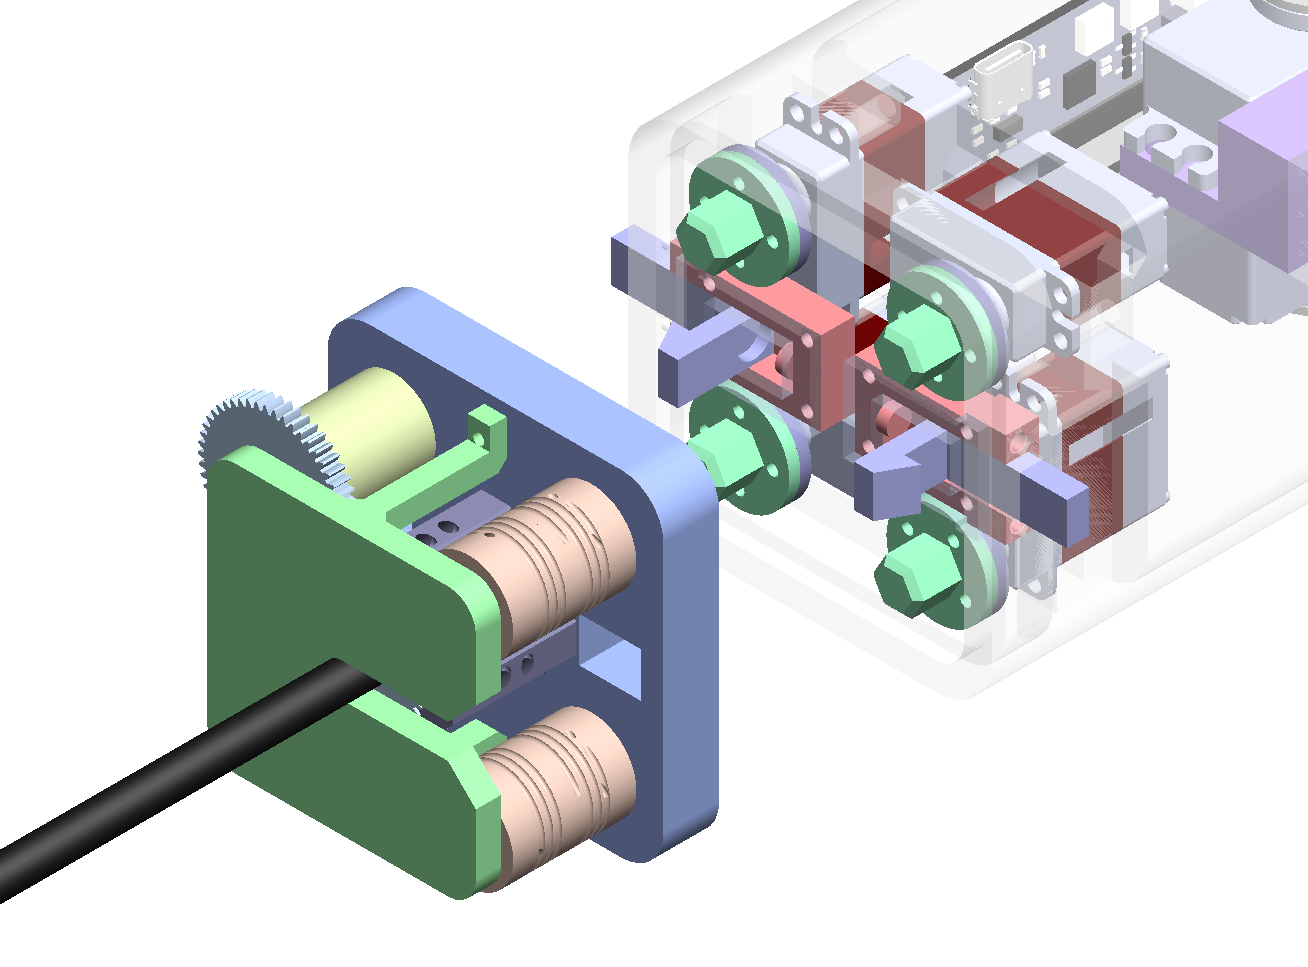
\includegraphics[width=0.7 \linewidth]{Figures/Motor Arrangement.png} 
    \caption{Motor Arrangement and Quick-Swap Mechanism}
    \label{fig:85}
\end{figure}
The quick-swap mechanism incorporates a user-friendly yet secure attachment scheme. Press-activated hooks are mounted within the main frame, enabling tool-free engagement and release. To attach a tip module, the user simply aligns and applies gentle pressure until the hooks audibly lock into place. For disengagement, bilateral release buttons must be depressed simultaneously while withdrawing the module. This dual-action release strategy prevents accidental detachment during operation, enhancing safety, while minimizing the number of steps required for module exchange.

This design ensures a robust mechanical and electrical connection during use, maintaining precise cable alignment and tension integrity while facilitating efficient tool interchange in time-sensitive surgical environments.

\subsection{Input Design}

The input module is designed to intuitively capture the user’s hand and finger motions with high precision and minimal latency. By integrating two STS3009 servos and two AS5600 magnetic encoders, the system is capable of sensing four degrees of freedom (DoFs): two DoFs from the wrist movement—yaw and pitch—and two DoFs from the fingers, namely roll and open/close actuation.

The wrist motions are translated through a dual-axis gimbal-like mechanism, where the STS3009 servos provide both actuation force and preliminary positional feedback. Fine rotational movements in yaw and pitch are accurately detected and relayed to the control system, enabling responsive and natural manipulation of the end-effector.
\begin{figure}[htbp]
    \centering
    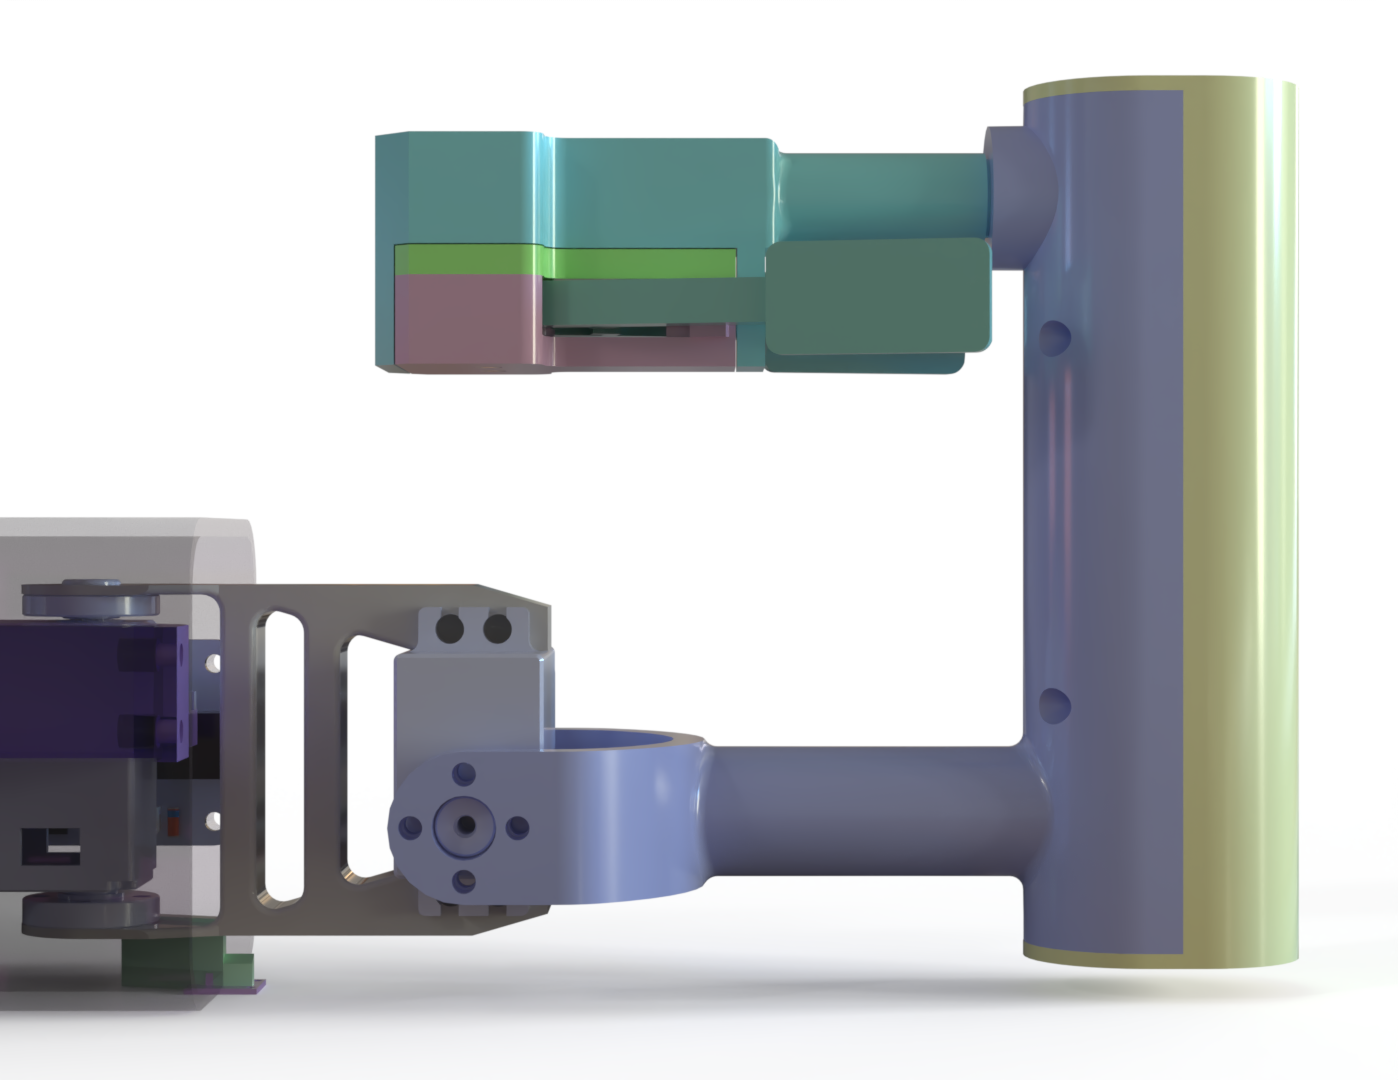
\includegraphics[width=0.7 \linewidth]{Figures/input.png} 
    \caption{Input Module Design}
    \label{fig:86}
\end{figure}
Finger actions are captured using the high-resolution AS5600 encoders, which detect both the rolling gesture and the degree of opening or closing of the fingers. Specifically, the open/close mechanism is implemented as an interchangeable module, allowing customization based on user preference or task requirements. The lever length and rebound force can be easily adjusted or swapped, facilitating ergonomic adaptability and reducing user fatigue during prolonged operations.

This modular and sensor-rich input design ensures that the system can accommodate a wide range of hand sizes and operating styles while maintaining accurate and reliable motion mapping between the user and the instrument.